%
% template.tex -- slide template
%
% (c) 2021 Prof Dr Andreas Müller, OST Ostschweizer Fachhochschule
%
\bgroup
\begin{frame}[t]
\setlength{\abovedisplayskip}{5pt}
\setlength{\belowdisplayskip}{5pt}
\frametitle{Frühere Seminare}
\vspace{-15pt}
\begin{columns}[t,onlytextwidth]
\begin{column}{0.44\textwidth}
\begin{center}
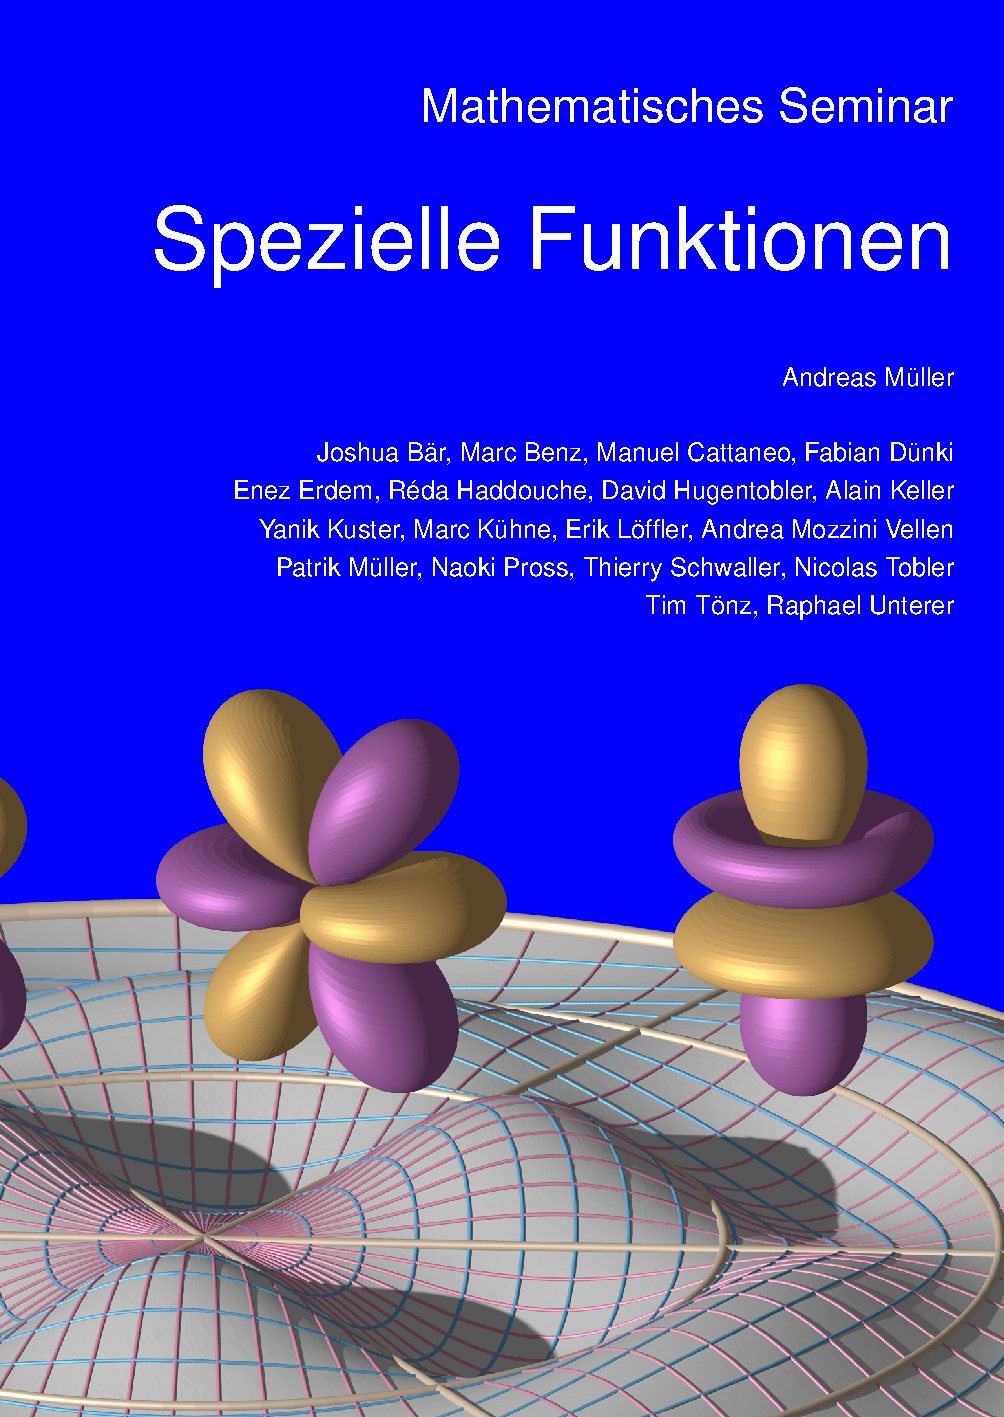
\includegraphics[width=\textwidth]{../slides/0/front.pdf}
\end{center}
\end{column}
\begin{column}{0.52\textwidth}
\begin{itemize}
\item {\color{gray}2024: Variationsrechnung}
\item {\color{gray}2023: Harmonische Analysis}
\item 2022: Spezielle Funktionen
\item 2021: Matrizen
\item 2020: Numerik
\item 2019: Wavelets
\item 2018: Klimawandel
\item 2017: Kosmologie
\item 2016: Differentialgleichungen
\item 2015: Quantenmechanik
\item 2014: High Performance Computing
\item 2013: Optimierung
\end{itemize}
{\color<2->{red}$\rightarrow$ Bibliothek}
\end{column}
\end{columns}
\end{frame}
\egroup
